\chapter{Charakterystyka EPUB}

\section{Omówienie}

EPUB jest standardem formatu dystrybucji cyfrowych publikacji i dokumentów opartych na standardach technologii webowej. EPUB definiuje
formę reprezentacji, organizacji struktury oraz kodowania określonej zawartości webowej, na co składają się XHTML, CSS, SVG, obrazy i
inne zasoby sprowadzone do formy pojedyńczego pliku. EPUB daje wydawcom możliwość stworzenia cyfrowej publikacji a następnie dystrybuowania
go, a odbiorcy łatwy dostęp do pliku niezależnie od urządzenia jakim operuje. Jako następca OEB (Open eBook Publication Structure),
zaprezentowanego w 1999 roku, EPUB 2 został ustandaryzowany w roku 2007 a aktualną jego wersją jest EPUB 3.1 (styczeń 2017). Dzisiaj jest
on standardem wykorzystywanym na szeroką skale przez wszystkich wydawców. Obok MOBI oraz PDF dominuje rynek, dzięki jego popularności
wsród wydawców oraz wsparciu urządzeń. W przeciwieństwie do MOBI które zostało spopularyzowane przez Amazon, właściciela sklepu amazon.com,
giganta dystybucji książek elektronicznych oraz producenta czytników elentronicznych marki Kindle, EPUB jest
standardem uniwersalnym, nieograniczonym do jednej platformy. EPUB zarówna jak i MOBI charakteryzuje się tym, że jego zawartość nie jest
statyczna, co oznacza, że ilość która jest wyświetlana dopasowana jest do wielkośći ekranu urządzenia dzięki czemu jest ona bardziej
przyjazna dla odbiorcy (PDF natomiast jest już podzielony na strony których nie da się podzielić). To co najbardziej różni EPUB od MOBI,
to wsparcie EPUB dla multimediów (od wersji 3.0) oraz CSS, który stulizuje cały dokument. Dzięki temu jest znacznie bardziej
elastyczny i nowoczesny. Popularną praktyką wśród dystrybutorów książek elektronicznych, jest dostarczanie ksiązki klientowi który ją
zakupił we wszystkich trzech wcześniej wymienionych formatach. EPUB jako standard jest szeroko udokumentowany dzięki International Digital
Publishing Forum\footnote{Adres url: \href{idpf.org}{idpf.org}}, grupie która nadrozuje rozwój formatu. W następnej sekcji zostanie
szczegółowo opisana struktura formatu EPUB.

\section{Specyfikacja}

Poniższa specyfikacja jest podzbiorem najważniejszych informacji wyselekcjonowanych ze specyfikacji EPUB 3.1 z dnia 5 stycznia 2017 roku
dostępnej na stronie International Digital Publishing Forum\footnote{Adres url najnowsej wersji specyfikacji: \href{http://www.idpf.org/epub3/latest}{http://www.idpf.org/epub3/latest}}.
Przedstawiono tutaj najbardziej istotne elementy formatu EPUB w celu zrozumienia problemu jakiego dotyczy projekt EPUBKit.

\subsection{EPUB Open Container Format}

\begin{figure}[ht!]
  \centering
  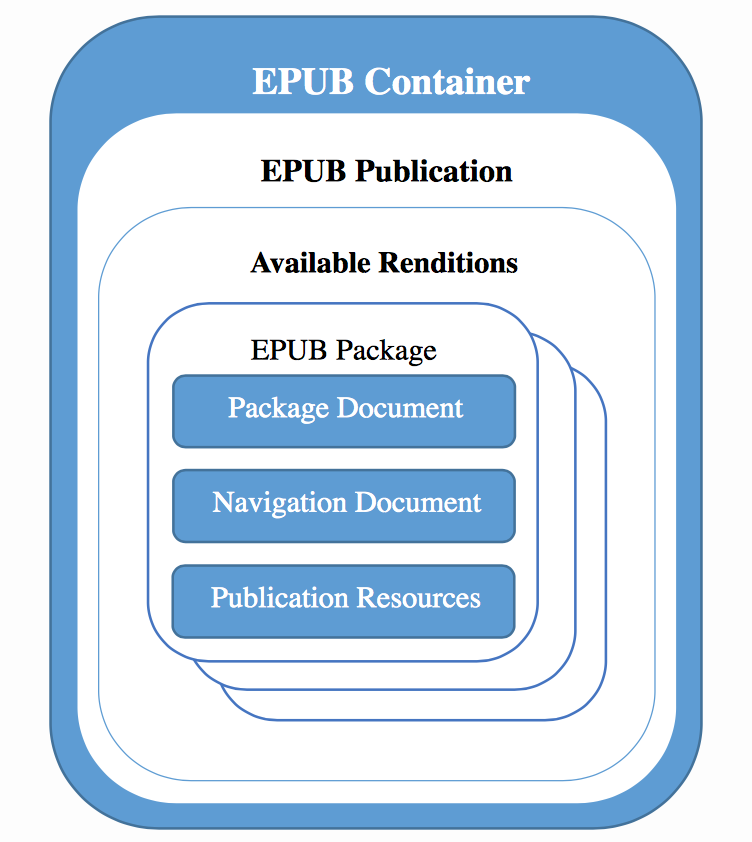
\includegraphics[width=.4\linewidth]{images/chapter-3-image-1-structure.png}
  \caption{Wizualna reprezentacja struktury formatu EPUB\cite{EPUBSpecificationRoadMap}.}
  \label{chapter-3-image-1-structure}
\end{figure}

Format EPUB definiuje jego najwyższy abstrakcyjny model jakim jest EPUB Publication. Model ten składa się z interpretacji jego zawartości.
Interpretacja która jest przedstawiona za pomocą EPUB Package zawiera już bezpośredniozawartość dokumenu, oraz poboczne zasoby mające
na celu wspomagać system czytający (z ang. ze specyfikacji "Reading System", jakim jest EPUBKit). Kluczowym elementem jest Package
Document który zawiera wszystkie metadane które są używane następnie przez system czytające do zaprezentowania publikacji użytkownikowi.
Zawiera on również kompletny manifest zasobów publikacji oraz "kręgosłup" (z ang. ze specyfikacji "Spine"), który reprezentuje sekwencję
w jakiej system czytający ma wyświetlać poszczególne elementy. EPUB Package zawiera również Navigation Document pełniący rolę spisu
treści, przeznaczony dla użytkownikowa do poruszania się po dokumencie. Wszystko to opakowane jest archiwum ZIP z rozszeżeniem ".epub".
Rozszeżenie informuje o charakterze pliku, oraz dostarcza infromacje o archimuw w ZIPowskim stylu za pomocą pliku "mimetype", oraz
zapewnia system o posiadaniu przez niego folderu "/META-INF" w krórym dostępny jest plik container.xml, niezbędny systemowi do określenia
lokalizacji zawartośći publikacji.

\begin{lstlisting}[caption={Przykładowy plik container.xml}, language=XML]
<?xml version="1.0" encoding="UTF-8"?>
<container version="1.0" xmlns="urn:oasis:names:tc:opendocument:xmlns:container">
    <rootfiles>
        <rootfile full-path="OEBPS/content.opf" media-type="application/oebps-package+xml"/>
   </rootfiles>
</container
\end{lstlisting}

To w jaki sposób zawartość publikacji jest zorganizowana określa standard EPUB Open Container Format (OPF), który definiuje reguły
enkapsulacji zasobów w pojedyńczym kontenerze abstrakcyjnym (EPUB Container) zawartym w archiwum ZIP. Struktura OPF to tylko jedna część
składająca się na EPUB Publication, druga część to zawartość przedstawiona urzytkownikowi która jest oparta o XHTML oraz (EPUB Content
Documents). Zawrtość ta jest rozszeżona o wiele dodatkowych zasobów potrzebnych do prawidłowego wyświetlenia publikacji jakimi mogą być
obrazy, pliki audio lub video, dodatkowe czcionki, skrypty oraz style nazywane w oficjalnej specyfikacji "EPUB Core Media Types".

\subsection{EPUB Content Documents}

Ta sekcja opisuje rolę jaką odgrywają standardów HTML, SVG i CSS w elektronicznej publikacji w formacie EPUB.
Wizualna kompozycja publikacji w znacznej mierze oparta jest o pliki XHTML. Specyfikacja EPUB Content Documents 3.1, szczegółowo opisuje
semantykę atrubutów wspieranych przez EPUB, które mają na celu wzbogacnie doświadczenia użytkownika. Artybuty te nadają dodatkową naturę
i znaczenie elementom XHTML, przy tym nie nadpisując ich pierwotnej funkcjonalności. Artybuty te są przeznaczonę wyłącznie dla systemów
czytających i przekazują istotne informacje odnośnie struktury i zawartości dokumentu.
Wsparcie standardu EPUB dla HTML nieodnosi się do konkretnej jego wersji, natomiast pozostawia tę kwestię twórcom systemów czytających.
To w ich obowiązkach leży upewnienie się, że każda publikacja zostanie prawidłowo przez system obsłużona.

\begin{lstlisting}[float=h, caption={Przykładowe wykorzystanie atrybutu epub:type aby oznaczyć zakończenie linii.\protect\cite{EPUBContentDocumentsSpecificationXML}}, language=XML]
<html ... xmlns:epub="http://www.idpf.org/2007/ops">
   ...
   <p> ... <span epub:type="pagebreak" title="234" id="p234"/> ... </p>
   ...
</html>
\end{lstlisting}

Kolejnym typem dokumentu ważnym dla formatu EPUB jest SVG (Scalable Vector Graphics). Coprawda uniwersalność XHTML przyczynia się do
tego iż jest to w znacznej mierze dominujący format przedstawiania treści w publikacji, SVG oferuje udogodnienia dzięki czemu również
znajuje zastosowanie. Format ten jest zazwyczaj wykorzystywany w specyficnych przypadkach, takich jak prezentacja zawartości publikacji
z gatunku manga czy komiks. Użytkownik oczekiwał by od tego typu dokumentu aby zawartość (w tym przypadku głównie graficzna) prezentowała
się dobrze na każdym urządzeniu, niezależnie od rozdzielczośći jego ekranu, i to właśnie SVG może zagwarantować. Dodatkowo, treść tych
dokumentów jest zazwyczaj z góry podzielona na strony, i narzuca systemom czytającym wyświelenie ich w określonej formie.

CSS odgrywa ogromną rolę w praktyce programistycznej (jako technologia webowa) od wielu lat, i jego możliwości wciąż rosną. Nietrudno się
domyślić że swoje miejsce CSS znaduje również w standardzie EPUB. Prezentacja publikacji jest sztywnie ustylizowana, chociaż nadpisywanie
stylu przez systemy czytające nie jest zabronione. Specyfikacja EPUB sugeruje, aby systemy dawały możliwość zmian w stylu publikacji
użytkownikowi, który dopasuje jej wygląd pod swoje upodobania. Zazwyczaj będzię to kolor tła, rozmiar czy typ czcionki. Specyfikacja również
przestrzega twórców publikacji w formacie EPUB aby rozważnie stylizować dokument. Niektóre systemy czytające mogą niewspierać pewnych
elementów CSS co może być problematyczne\cite{EPUBContentDocumentsSpecificationCSS}.

To o czym również należy wspomnieć opisując EPUB Content Documents jest to, że EPUB wspiera skrypty w dokumentach HTML czy SVG. Opcjonalne
jest wspieranie skryptowania w systemach czytających, natomiast te systemy które wspierają skryptowane dokumenty, muszą wziąć pod uwagę
pewne niebezpieczeństwa z tym związane. Specyfikacja przestrzega, aby systemy czytające zapewniały izolację publikacji w celu uniknięcia
niebezpieczeństw zagraząjącym podatnej na ataki zawartości. System powinien monitorować wszelkie aktywności aby zawartość pozostała
nienaruszona. Należy założyć, że może zostać przeprowadzony atak na zawartość innych plików w strukturze publikacji, atak na sam system
czytający (np. próba zdobycia danych użytkownika), atak na sieć czy wszczepianie innych złośliwych skryptów w niezaszyfrowane fragmenty
dokumentu. Ponadto systemy które zezwalają na stałe przechowywanie publikacji, muszę dostarczyć metody zezwalające podgląd i kasowanie
danych publikacji. W sytuacji usunięcia publikacji przez użytkownika, system musi skasować wszelakie pliki z nią związane\cite{EPUBContentDocumentsSpecificationJS}.

\subsection{EPUB Core Media Types}

Zaobserwować można, że EPUB jako format jest bardzo ściśle uspecyfikowany odnośnie jego struktury i wspieranych technologii. W przypadku
samej zawartości nie jest inaczej. Specyfikacja EPUB 3 Core Media Types\footnote{Adres url: \href{https://idpf.github.io/epub-cmt/v3/}{https://idpf.github.io/epub-cmt/v3/}}
szczegółowo opisuje jakie typy mediów mogą zostać załączone do publikacji, i określa dla nich unikalny typ (Media Type) który jest
wykorzystywany w celach poinformowania systemu czytającego o typie danego elementu. Ta sekcja opisuje poszczególne typy mediów wspierane
przez EPUB, niezagłębiając sie przy tym w techniczne szczegóły konkretnego typu.

\subsubsection*{Image Types}

Wspierane typy obrazów (Image Types) to GIF, JPEG, PNG oraz SVG. Ich typy zadeklarowane w standarcie EPUB to kolejno "image/gif", "image/jpeg",
"image/png", "image/svg+xml". Notacja ta wykorzystywana jest w atrybutach elementów nawiązujących (wskazujących na/deklarujących) konktetny
obiekt odpowiedniego typu. Oznaczenia te możemy spotkać w manifescie publikacji.

\begin{lstlisting}[caption={Przykładowy fragment manifestu znajdującego się w pliku content.opf}, language=XML]
<manifest>
  ...
  <item href="Images/image-1.jpg" id="id1" media-type="image/jpeg"/>
  <item href="Images/image-2.jpg" id="id2" media-type="image/jpeg"/>
  ...
</manifest>
\end{lstlisting}

Ten sposób oznacznia elementów wykorzystywany jest w deklarowaniu każdego obiektu o wspierany przez EPUB typie.

\subsubsection*{Audio Types}

EPUB wspiera pliki audio w formacie MP3("audio/mpeg") oraz MP4("audio/mp4"). Zapewne zdecydowano się na te dwa konktetne standardy ze
względy na ich popularnośc oraz mały rozmiar dzięki stosunkowo wysokiej kompresji.

\subsubsection*{Video Types}

Ze względu na rozbieżność preferecji wśród autorów oraz twórców specyfikacji, EPUB nie definuje preferowanego typu wideo dla publikacji
w swoim standardzie. IDPF proponuje dwa formaty kodowania, H.264 oraz WebM ale nie kładzie nacisku na jeden z nich, tę kwestię pozostawia
na ten moment autorom. Spór dotyczący określenia konkretnego formatu plików wideo rozchodzi się o szerokie wsparcie H.264 przeciwko
nieopatentowanemu, wolnemu formatowi WebM, który jednak wciąż nie jest spopularyzowanym standardem. IDPF deklaruje, że najprawdopodobniej
w penym momencie preferowany standard zostanie określony, jednakże teraz jest jeszcze na to zbyt wcześnie\cite{WhatIsEPUB3Video}.

\subsubsection*{Application, Text, Font Types}

Pozostałe typy które wspiera EPUB zdecydowano się opisać razem w tej sekcji w skrócie ze względu na to, że wszystkie przysłużają się
jednemu celowi jakim jest prezentacja treści. Są to czcionki w formacie WOFF("application/font-woff"), WOFF2("font/woff2") oraz
OpenType/TrueType("application/font-sfnt"), pliki CSS("text/css"), skrypty("application/javascript"), dokumenty XHTML("application/xhtml+xml"),
nawigacyjne pliki NCX("application/x-dtbncx+xml") oraz nakładki MediaOverlays3("application/smil+xml") wraz z plikami PLS("application/pls+xml"),
które mają na celu odtworzenia tekstu w formie dźwiękowej\cite{EPUBCoreMediaTypes}.

\subsubsection*{Foreign Resources}

Należy wspomnieć iż EPUB zezwala na użycie niewspieranych formatów, jednakże nie gwarantuje, że zostaną prawidłowo obsłużone przez systemy
czytające, od których wymaga jedynie wsparcia na wcześniej wymienionych formatów. W przypadku użycia przez autora publikacji niewspieranych
formatów, specyfikacja EPUB wymaga od niego zadeklarowanie tak zwanego "Core Media Type fallback", czyli typu wspieranego który zastępczo będzie
przypisany do obiektu jeżeli system czytający nie bedzię wspirał pierwotnie wskazanego typu\cite{EPUBSpecificationForeignResources}.
